% Figure M9-interp hero: interpretability-first companion to M9 scRNA.
% Generated by experiments/m9_scrna.py --interpretability.
\begin{figure}[t]
 \centering
 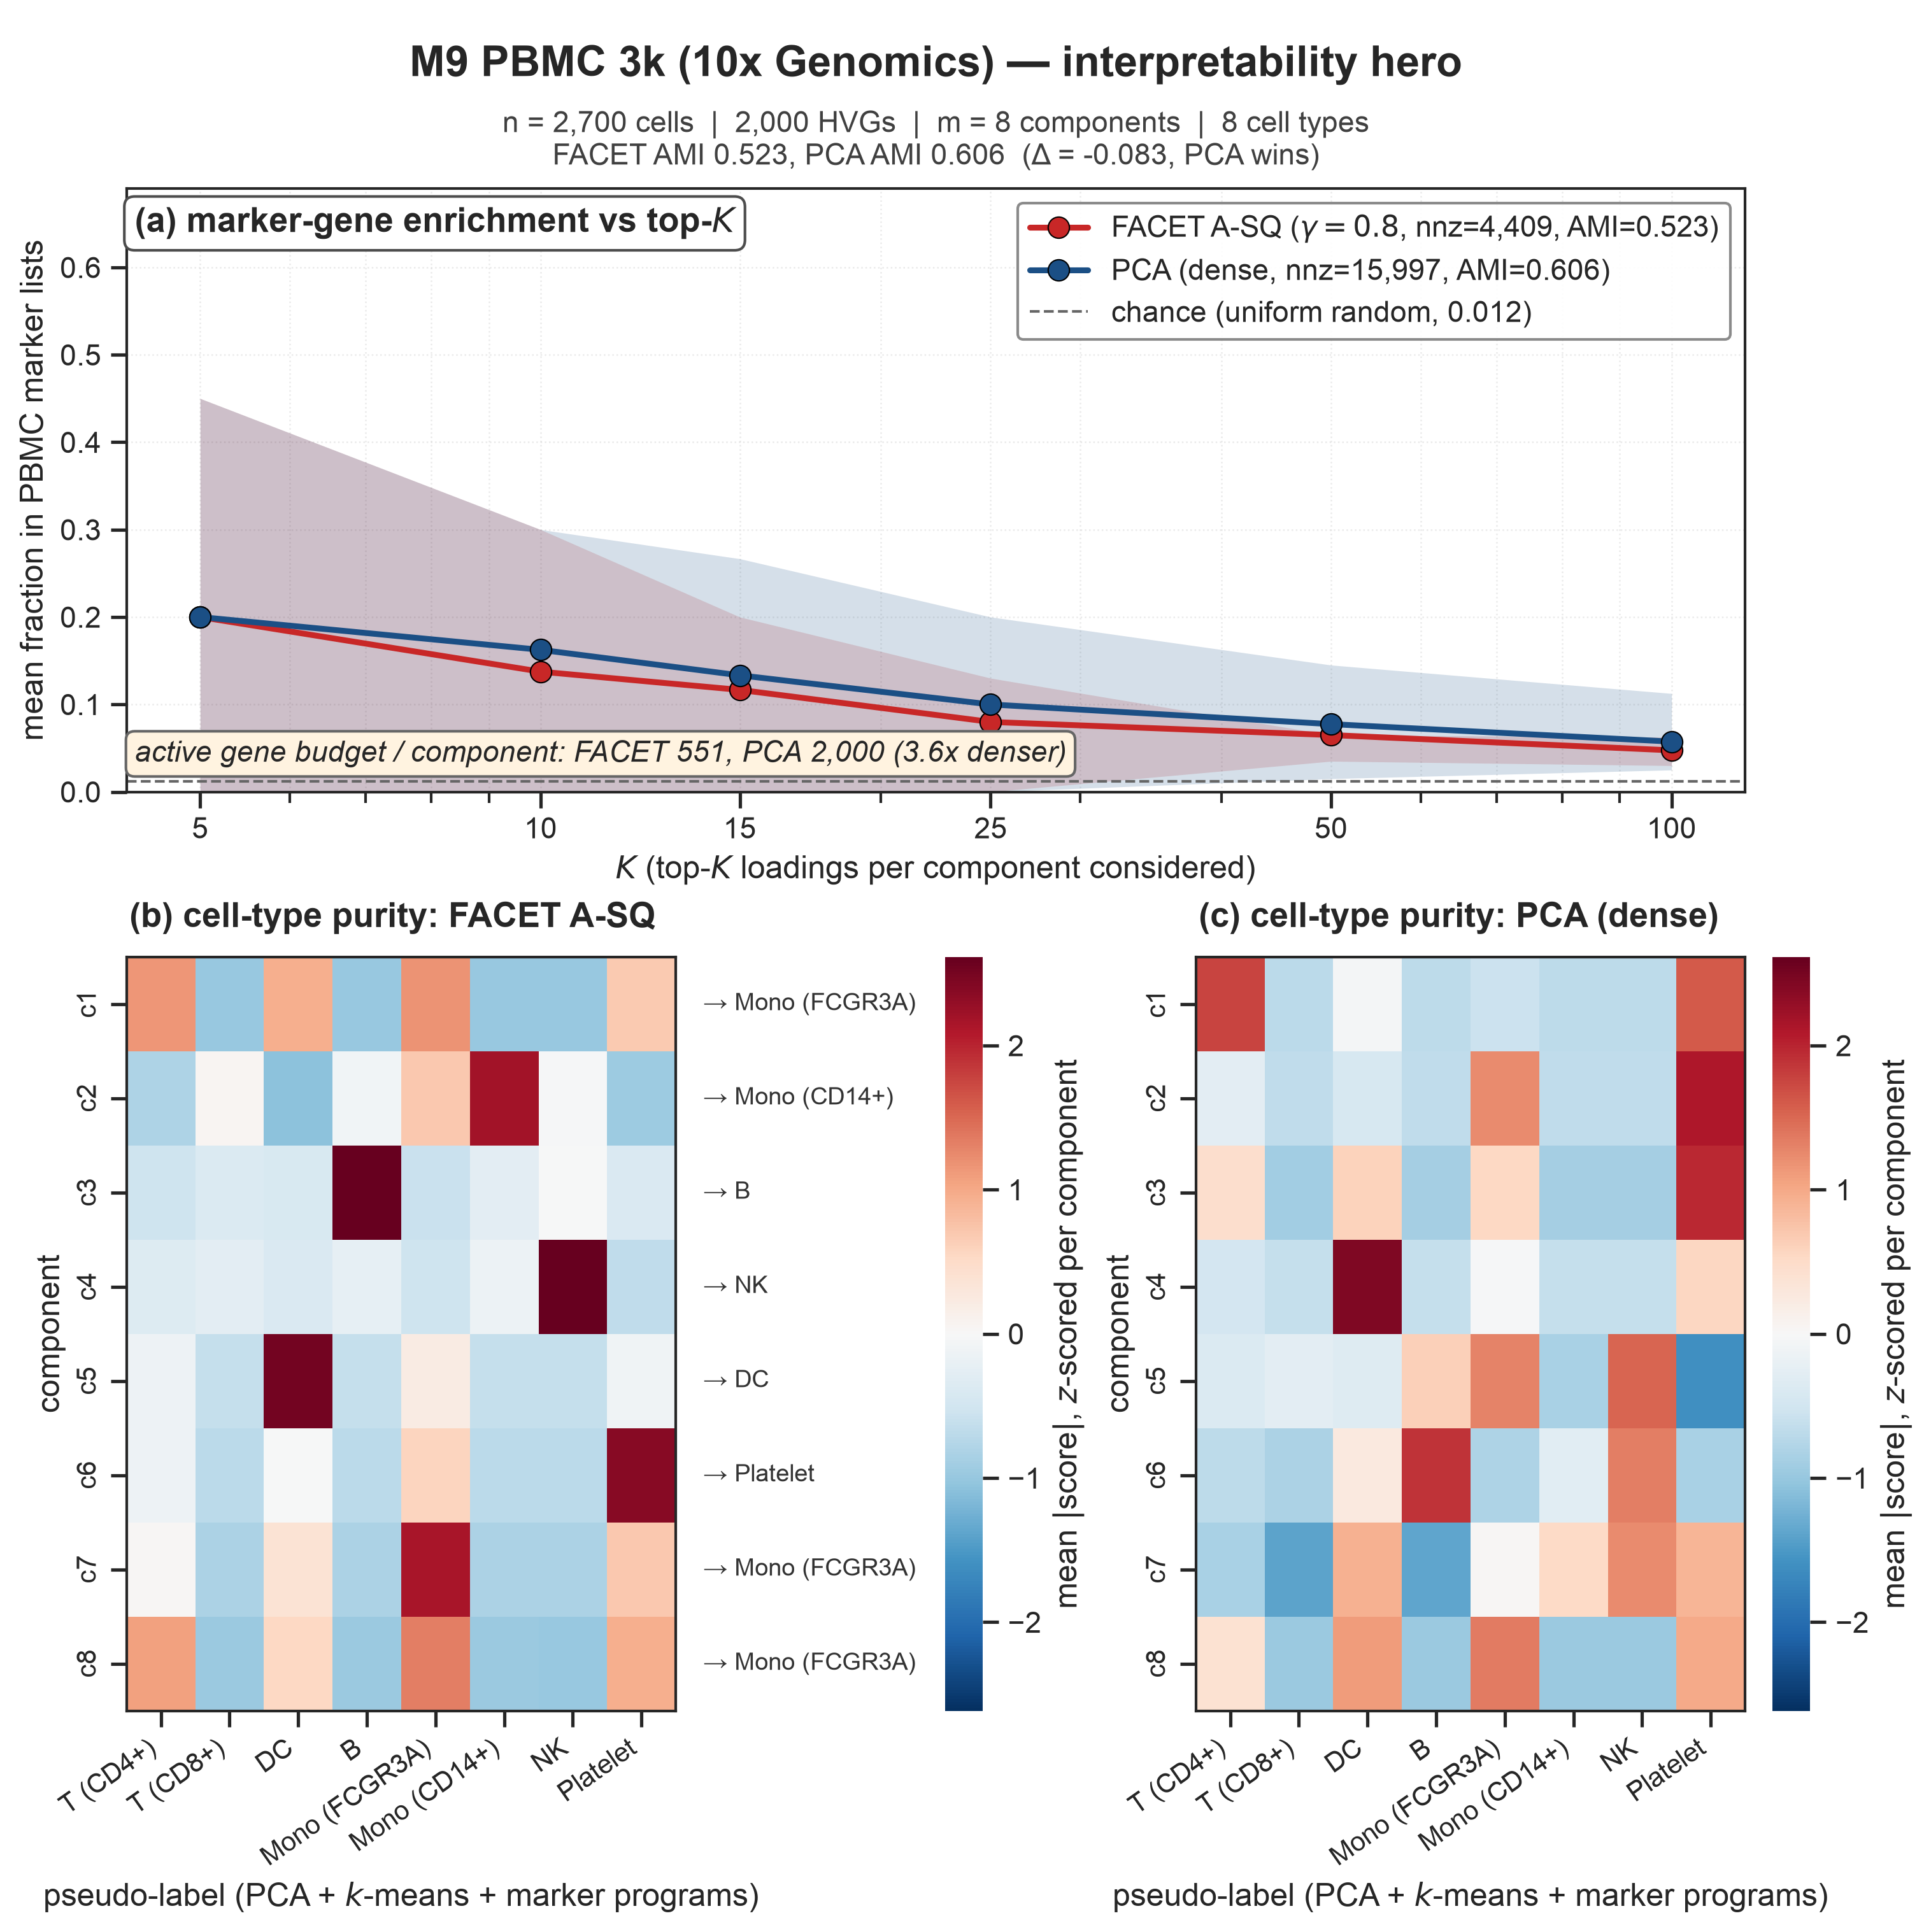
\includegraphics[width=\linewidth]{../shared/figures/generated/m9_scrna_interpretability_hero.png}
 \caption{\textbf{M9 interpretability hero: PBMC 3k with pseudo-labels.} Same 2{,}700 PBMCs $\times$ 2{,}000 HVGs as Fig.~\ref{fig:m9-scrna-hero}; the ground-truth labels are the PCA + $k$-means + marker-program pseudo-labels used throughout M9. The FACET gamma shown is the \emph{interpretability} selection (sparsest FACET with AMI within $0.025$ of the max-AMI FACET), not the max-AMI gamma. \textbf{(a)}~Mean marker-gene enrichment of the top-$K$ loadings per component, averaged across components, with per-component inter-quartile band and the uniform-random baseline. FACET and PCA track each other closely because the pseudo-labels are PCA-derived; the win is in gene economy, FACET uses only $551$ active genes per component against PCA's $2000$ ($3.6\times$ denser). \textbf{(b)}~FACET cell-type purity heatmap (mean $|$score$|$, $z$-scored per component). Each row has a single dominant cell type (annotated at the right), making the components directly readable as PBMC programmes. \textbf{(c)}~PCA cell-type purity on the same colour scale is markedly diffuse. The pseudo-label caveat is relaxed on native labels in Figs.~\ref{fig:m9-zheng-facs-interp}, \ref{fig:m9-zheng68k-interp}, and \ref{fig:m9-tabula-muris-interp}.}
 \label{fig:m9-scrna-interp}
\end{figure}
